\documentclass[11pt,a4paper]{article}

\usepackage[utf8]{inputenc}
\usepackage[T1]{fontenc}
\usepackage[english]{babel}
\usepackage{lmodern}
\usepackage[margin=2.2cm]{geometry}
\usepackage{enumitem}
\usepackage{xcolor}
\usepackage[most]{tcolorbox}
\usepackage{booktabs}
\usepackage{tabularx}
\usepackage{array}
\usepackage{tikz}
\usetikzlibrary{arrows.meta, positioning, calc, decorations.markings}
\usepackage[hidelinks]{hyperref}

\definecolor{accent}{RGB}{0,90,150}
\definecolor{good}{RGB}{0,130,60}
\definecolor{bad}{RGB}{190,40,40}
\definecolor{mid}{RGB}{200,120,0}

\newcommand{\yes}{\textcolor{good}{\textbf{Yes}}}
\newcommand{\no}{\textcolor{bad}{\textbf{No}}}
\newcommand{\partly}[1]{\textcolor{mid}{\textbf{#1}}}

\newtcolorbox{answer}{
  colback=accent!4, colframe=accent!60!black, boxrule=0.5pt, arc=2pt,
  left=6pt, right=6pt, top=4pt, bottom=4pt
}

\newcolumntype{L}{>{\raggedright\arraybackslash}X}

\setlength{\parindent}{0pt}
\setlength{\parskip}{0.45em}

\tikzset{
  phase/.style={draw=accent!70!black, fill=accent!10, rounded corners=2pt,
                minimum width=3.3cm, minimum height=0.8cm, font=\small, align=center},
  test/.style={draw=good!70!black, fill=good!10, rounded corners=2pt,
               minimum width=3.3cm, minimum height=0.8cm, font=\small, align=center},
  flow/.style={-{Stealth[length=2.5mm]}, thick},
  link/.style={{Stealth[length=2mm]}-{Stealth[length=2mm]}, dashed, gray}
}

\title{\textbf{Lab 1 -- Section I: Software Development Process Models}\\[0.3em]
\large Software Engineering -- Case Study: Campus Mobility App}
\author{Roman Benz}
\date{\today}

\begin{document}
\maketitle

%====================================================================
\section{Software Development Life Cycle}

\subsection*{Assignment of the activities to SDLC phases}

\begin{tabularx}{\textwidth}{@{}c L l@{}}
\toprule
\textbf{Act.} & \textbf{Description} & \textbf{SDLC phase} \\
\midrule
C & Team determines what functionality students need & Requirements Engineering \\
E & Architects define components and interfaces      & Design \\
A & Developers implement the connection search        & Implementation \\
G & Testers check the app against the specified requirements & Testing (system test) \\
B & Students check whether the app meets their expectations  & Testing (acceptance test) \\
D & Release to the university app store               & Deployment \\
F & Fixing defects and adapting after release         & Maintenance \\
\bottomrule
\end{tabularx}

\subsection*{Reasonable order}

\begin{answer}
\centering
\textbf{C} $\rightarrow$ \textbf{E} $\rightarrow$ \textbf{A} $\rightarrow$
\textbf{G} $\rightarrow$ \textbf{B} $\rightarrow$ \textbf{D} $\rightarrow$
\textbf{F}
\end{answer}

The system test (G) comes before the acceptance test (B): the team first
verifies internally that the specification is fulfilled before real users
validate whether the app fits their needs. Maintenance (F) is only possible
after the release (D).

\subsection*{Typical artifacts}

\begin{tabularx}{\textwidth}{@{}l L@{}}
\toprule
\textbf{Activity} & \textbf{Typical artifact} \\
\midrule
Requirements Engineering & Requirements specification (e.g.\ list of
  functional / non-functional requirements, user stories, use case diagram) \\
Design & Architecture / component diagram, interface specification
  (e.g.\ API of the timetable service), data model \\
Implementation & Source code, executable build (app package), code
  documentation \\
Testing & Test plan and test cases, test report, defect / bug reports \\
\bottomrule
\end{tabularx}

%====================================================================
\section{Waterfall Model}

\subsection*{Simplified Waterfall Model}

\begin{center}
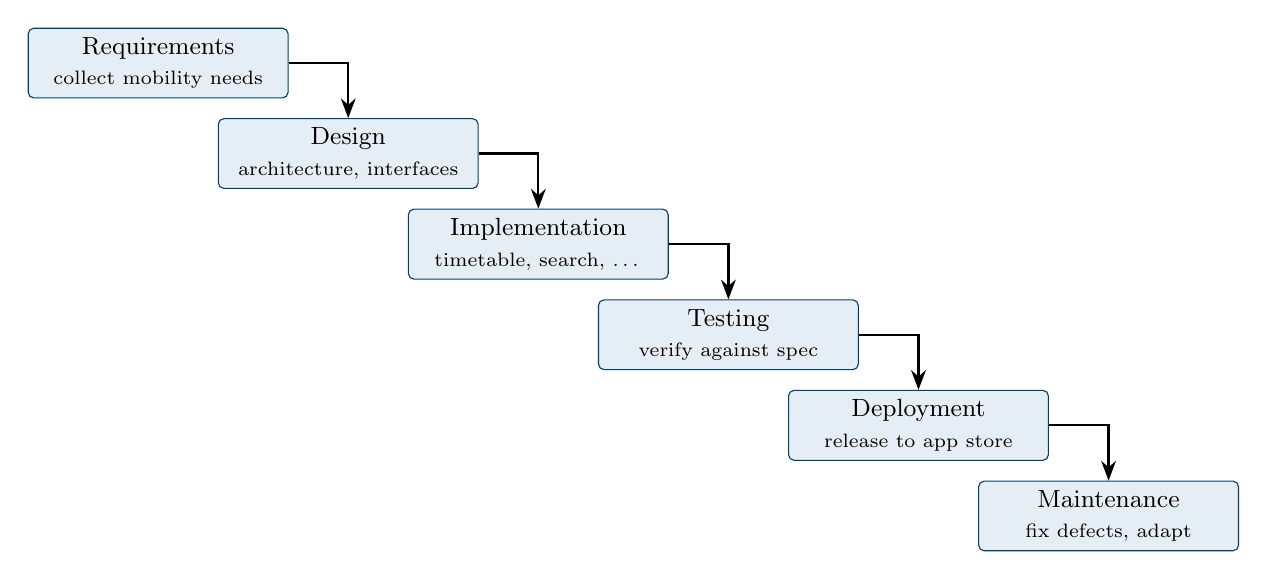
\begin{tikzpicture}[node distance=0.25cm and -0.9cm]
  \node[phase] (req) {Requirements\\\scriptsize collect mobility needs};
  \node[phase, below right=of req] (des) {Design\\\scriptsize architecture, interfaces};
  \node[phase, below right=of des] (imp) {Implementation\\\scriptsize timetable, search, \dots};
  \node[phase, below right=of imp] (tst) {Testing\\\scriptsize verify against spec};
  \node[phase, below right=of tst] (dep) {Deployment\\\scriptsize release to app store};
  \node[phase, below right=of dep] (mnt) {Maintenance\\\scriptsize fix defects, adapt};
  \foreach \a/\b in {req/des, des/imp, imp/tst, tst/dep, dep/mnt}
    \draw[flow] (\a.east) -| (\b.north);
\end{tikzpicture}
\end{center}

\begin{tabularx}{\textwidth}{@{}l L@{}}
\toprule
\textbf{Phase} & \textbf{Activities for the Campus Mobility App} \\
\midrule
Requirements   & Specify shuttle overview, departure/arrival times, connection
                 search, delay notifications, favorites \\
Design         & Define app architecture, backend for timetable data,
                 notification service, data model, interfaces \\
Implementation & Program all features of the specification \\
Testing        & Unit, integration and system tests against the specification \\
Deployment     & Publish the app in the university app store \\
Maintenance    & Bug fixes, adaptations (e.g.\ new OS versions) \\
\bottomrule
\end{tabularx}

\subsection*{When does the Waterfall Model work well?}

If the university's requirements are stable and well understood, every
phase can be completed fully, documented and reviewed before the next one
starts. The scope is known in advance, so cost, schedule and staffing can
be planned reliably. There is little need to go back to an earlier phase,
which is exactly the assumption the Waterfall Model is built on.

\subsection*{Problem: late request for public transport integration}

In the Waterfall Model, requirements and design are considered
\emph{finished} once implementation starts. The new requirement means:
\begin{itemize}[itemsep=0.1em]
  \item going back to requirements \emph{and} design -- the architecture
        must now include an external data source (public transport API),
        new interfaces and a different data model;
  \item already implemented parts (especially the connection search) may
        have to be reworked, and test plans must be changed;
  \item the change costs much more the later it occurs, and schedule and
        budget no longer fit. The model has no built-in mechanism for
        handling changes.
\end{itemize}

\subsection*{Advantages and disadvantages for this project}

\begin{tabularx}{\textwidth}{@{}L L@{}}
\toprule
\textbf{Advantages} & \textbf{Disadvantages} \\
\midrule
Clear, easy-to-understand structure with defined milestones and
documentation for every phase. &
Changes (e.g.\ public transport integration, planned future features) are
expensive and hard to include. \\
Good plannability of cost and schedule when the requirements are stable. &
Students see working software only at the very end, so feedback and
detected misunderstandings come very late. \\
\bottomrule
\end{tabularx}

%====================================================================
\section{V-Model}

\subsection*{Simplified V-Model}

\begin{center}
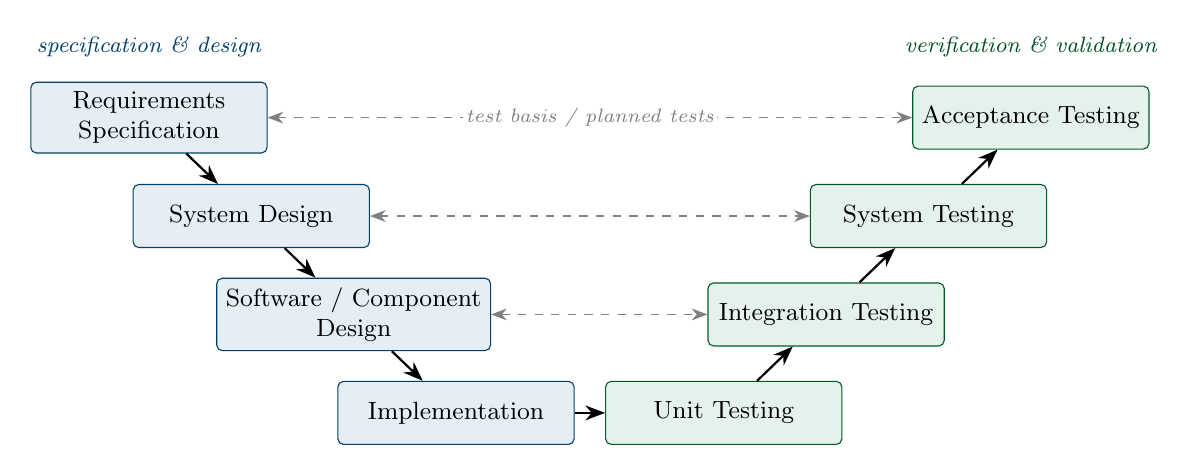
\begin{tikzpicture}[x=1cm, y=1cm,
    phase/.append style={minimum width=3.0cm},
    test/.append style={minimum width=3.0cm}]
  % left side: specification and design
  \node[phase] (rs) at (0,0)      {Requirements\\Specification};
  \node[phase] (sd) at (1.3,-1.25) {System Design};
  \node[phase] (cd) at (2.6,-2.5)  {Software / Component\\Design};
  \node[phase] (im) at (3.9,-3.75) {Implementation};
  % right side: test levels (same height as their counterpart)
  \node[test] (ut) at (7.3,-3.75)  {Unit Testing};
  \node[test] (it) at (8.6,-2.5)   {Integration Testing};
  \node[test] (st) at (9.9,-1.25)  {System Testing};
  \node[test] (at) at (11.2,0)     {Acceptance Testing};

  \draw[flow] (rs) -- (sd);
  \draw[flow] (sd) -- (cd);
  \draw[flow] (cd) -- (im);
  \draw[flow] (im) -- (ut);
  \draw[flow] (ut) -- (it);
  \draw[flow] (it) -- (st);
  \draw[flow] (st) -- (at);

  % correspondences
  \draw[link] (rs.east) -- (at.west);
  \draw[link] (sd.east) -- (st.west);
  \draw[link] (cd.east) -- (it.west);

  \node[font=\footnotesize\itshape, text=accent!70!black] at (0,0.9)
    {specification \& design};
  \node[font=\footnotesize\itshape, text=good!60!black] at (11.2,0.9)
    {verification \& validation};
  \node[font=\scriptsize\itshape, text=gray, fill=white, inner sep=1pt]
    at (5.6,0) {test basis / planned tests};
\end{tikzpicture}
\end{center}

\subsection*{Assignment of the test levels}

\begin{tabularx}{\textwidth}{@{}l l L@{}}
\toprule
\textbf{Development activity} & \textbf{Test level} & \textbf{What is checked?} \\
\midrule
Requirements Specification  & Acceptance Testing  & Does the app meet the
  students' / university's needs? \\
System Design               & System Testing      & Does the complete system
  behave as specified? \\
Software / Component Design & Integration Testing & Do components (e.g.\
  search, timetable service, notifications) work together via their
  interfaces? \\
Implementation              & Unit Testing        & Does each unit (e.g.\
  search algorithm) work correctly? \\
\bottomrule
\end{tabularx}

\subsection*{Meaning of the connection between both sides}

The horizontal connections (dashed; for implementation and unit testing the bottom of the V) show that every specification level on the
left is the \emph{test basis} for one test level on the right. The tests
are \emph{planned already} when the corresponding specification is
written (e.g.\ acceptance tests while writing the requirements), and later
they check whether the result of that level was fulfilled. This makes the
relationship between development artifacts and tests explicit and
traceable.

%====================================================================
\section{Iterative and Incremental Development}

\subsection*{Three increments}

\begin{tabularx}{\textwidth}{@{}c p{4.6cm} L@{}}
\toprule
\textbf{Inc.} & \textbf{Functionality} & \textbf{Value for the users} \\
\midrule
1 & Shuttle timetable, connection search &
  Core function: students see shuttles and departure/arrival times and can
  find a connection between university locations. \\
2 & Delay notifications, favorites &
  More reliable and more comfortable: students are informed about delays
  and can reuse their daily routes with one tap. \\
3 & Public transport integration, bicycle sharing, parking information &
  The app becomes a complete campus mobility platform covering all means
  of transport. \\
\bottomrule
\end{tabularx}

\subsection*{Why is the first increment already useful?}

It covers the main purpose of the app: getting from one university
location to another by shuttle. With timetable and connection search,
students can already plan real trips. All further features (notifications,
favorites, other means of transport) only make this core function more
comfortable or broader. In addition, the first increment provides early
feedback from real users for the following increments.

\subsection*{Increment vs.\ iteration}

\begin{answer}
\begin{itemize}[leftmargin=1.2em, itemsep=0.15em]
  \item \textbf{Increment:} a \emph{usable extension} of the product -- new
        functionality is added (``building the product piece by piece'').
  \item \textbf{Iteration:} a \emph{repeated development cycle} (plan,
        build, test, evaluate) in which existing parts are reworked and
        improved (``improving the product step by step'').
\end{itemize}
\end{answer}

\subsection*{Evolution of the connection search}

This is \textbf{primarily iterative development}: the \emph{same} feature
(connection search) is revisited and refined in each version -- first a
basic search, then delay-aware, then multimodal. The feature already exists
from version 1 and is improved repeatedly.

There is also an incremental aspect: version 3 adds visible new
functionality (public transport). But the main focus is the step-by-step
refinement of one existing feature, so ``iterative'' fits better.

%====================================================================
\section{Spiral Model}

\subsection*{Why is the Spiral Model suitable?}

The delay prediction is a high-risk feature: the team has no experience
with machine learning prediction systems and it is unknown whether the GPS
data is good enough. The Spiral Model is \emph{risk-driven}: in each cycle,
the biggest risks are identified first and reduced with prototypes or
experiments, before more effort is invested. This way, the team can find
out early -- and cheaply -- whether the feature is feasible, and can still
change direction or stop.

\subsection*{Two project risks}

\begin{enumerate}[itemsep=0.1em]
  \item \textbf{Data quality:} GPS data may be inaccurate, incomplete,
        delayed or missing (e.g.\ signal loss, sending intervals too long).
  \item \textbf{Prediction quality / know-how:} the ML model may not be
        accurate enough to be useful, and the team lacks experience in
        building and operating such a model (effort and schedule are hard
        to estimate).
\end{enumerate}

\subsection*{Investigating the data-quality risk in an early spiral}

\begin{enumerate}[itemsep=0.1em]
  \item Record GPS data of a few shuttles for some weeks together with the
        real departure/arrival times.
  \item Analyse the data: accuracy, update frequency, gaps and outliers.
  \item Build a simple prototype (e.g.\ a baseline model or a simple
        regression) and compare predicted delays with the real ones.
  \item Decide based on the result: continue with the approach, improve
        the data source (e.g.\ better GPS hardware), or drop the feature.
\end{enumerate}

\subsection*{Activities of one spiral cycle}

\begin{center}
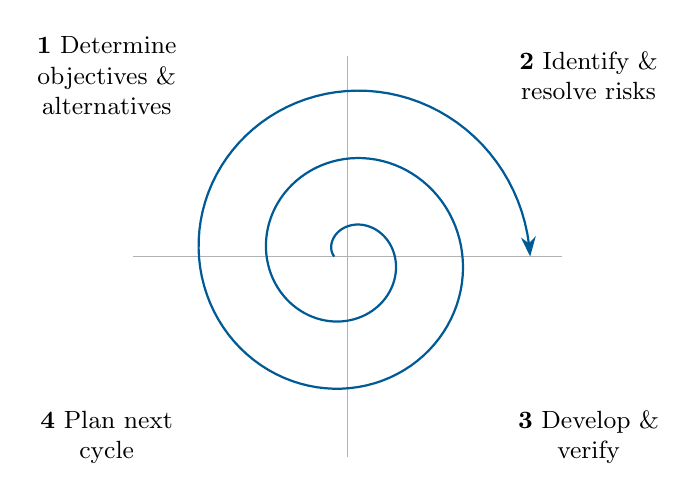
\begin{tikzpicture}[scale=0.85, every node/.style={font=\small}]
  \draw[gray!60] (-3.2,0) -- (3.2,0);
  \draw[gray!60] (0,-3.0) -- (0,3.0);
  \draw[accent, thick, -{Stealth[length=2.5mm]}, domain=0:900, samples=250, variable=\t]
    plot ({-(0.2+0.0028*\t)*cos(\t)}, {(0.2+0.0028*\t)*sin(\t)});
  \node[align=center] at (-3.6,2.7) {\textbf{1} Determine\\objectives \&\\alternatives};
  \node[align=center] at (3.6,2.7)  {\textbf{2} Identify \&\\resolve risks};
  \node[align=center] at (3.6,-2.7) {\textbf{3} Develop \&\\verify};
  \node[align=center] at (-3.6,-2.7){\textbf{4} Plan next\\cycle};
\end{tikzpicture}
\end{center}

\begin{tabularx}{\textwidth}{@{}l L@{}}
\toprule
\textbf{Activity} & \textbf{Explanation} \\
\midrule
1. Determine objectives, alternatives, constraints &
  What should this cycle achieve? Which solution approaches are possible
  (e.g.\ different prediction methods)? \\
2. Identify and resolve risks &
  Evaluate the alternatives regarding their risks and reduce the biggest
  risks, e.g.\ with prototypes, simulations or analyses. \\
3. Develop and verify &
  Develop and test the (partial) product of this cycle, e.g.\ a prototype
  or a feature. \\
4. Plan the next cycle &
  Review the results with stakeholders and decide whether and how to
  continue (next cycle, change of direction, or stop). \\
\bottomrule
\end{tabularx}

%====================================================================
\section{Identify the Process Model}

\begin{tabularx}{\textwidth}{@{}c l L@{}}
\toprule
\textbf{Scen.} & \textbf{Process model} & \textbf{Supporting characteristic} \\
\midrule
A & V-Model &
  ``For every specification level, a corresponding test level is
  planned'' and the traceability between artifacts and tests is
  documented. \\
B & Iterative / Incremental &
  ``A small but usable version is released first'', then functionality is
  added and existing functionality is continuously improved. \\
C & Spiral Model &
  New, unknown technologies; prototypes are built ``to investigate
  technical risks'' before the final architecture is fixed. \\
D & Waterfall Model &
  Detailed and stable specification at the start; all phases are performed
  ``largely sequentially''. \\
\bottomrule
\end{tabularx}

%====================================================================
\section{Final Comparison}

\begin{center}
\renewcommand{\arraystretch}{1.35}
\small
\begin{tabularx}{\textwidth}{@{}>{\raggedright\arraybackslash}p{4.3cm}
  >{\centering\arraybackslash}X >{\centering\arraybackslash}X
  >{\centering\arraybackslash}X >{\centering\arraybackslash}X@{}}
\toprule
\textbf{Characteristic} & \textbf{Waterfall} & \textbf{V-Model} &
\textbf{Iterative / Incremental} & \textbf{Spiral} \\
\midrule
Development mainly sequential? & \yes & \yes & \no & \no \\
Explicit relationship between development and testing? &
  \partly{Limited} & \yes & \partly{Not central} & \partly{Not central} \\
Early delivery of partial functionality possible? &
  \no & \no & \yes & \partly{Possible} \\
Explicit focus on risk analysis? & \no & \no & \partly{Not necessarily} & \yes \\
Well suited to changing requirements? &
  \no & \partly{Limited} & \yes & \yes \\
\bottomrule
\end{tabularx}
\end{center}

\textbf{Notes:}
\begin{itemize}[itemsep=0.1em]
  \item \emph{Waterfall} does have a test phase, but it is not explicitly
        linked to the individual specification levels -- that is the main
        addition of the \emph{V-Model}.
  \item In the \emph{Spiral Model}, each cycle produces a (partial)
        product, so early partial delivery is possible, but its focus is
        risk reduction rather than delivering usable increments.
  \item \emph{Iterative / incremental} development handles changing
        requirements well because each new iteration or increment can take
        the latest requirements into account.
\end{itemize}

\end{document}
